\section{Results – Strategy S4: Multi-LLM Per-Field}
\label{sec:eval-s4}

The \textbf{S4: Multi-LLM Per-Field} strategy applies consensus at the slot level: each field is extracted by multiple models and consolidated via a field-aware verifier. We evaluate three variants: \textbf{S4.0} without few-shot prompting on the original MUC-4 dataset, \textbf{S4.1} with few-shot prompting on the original dataset, and \textbf{S4.2} with few-shot prompting on a speech-style variant.

Figure~\ref{fig:s4-variants-bar} shows that per-field consensus behaves markedly differently from the full-document strategies. All three variants achieve high NES ($\geq 0.612$) while exhibiting \emph{negative} EAI (down to $-0.080$ in S4.0), which means that S4 performs very well when gold labels are nonempty but tends to overfill when gold is empty. This pattern is reflected in the combination of high hallucination rates (HR between $0.476$ and $0.551$) and very low missing rates (MR between $0.112$ and $0.150$): the verifier prefers to output something rather than abstain. Introducing few-shot prompting (S4.1 vs.\ S4.0) slightly increases OBS (from $0.549$ to $0.579$) and SF1 (from $0.589$ to $0.613$), raises FDA (from $0.693$ to $0.709$), and reduces HR (from $0.551$ to $0.476$) at the cost of a modest MR increase (from $0.112$ to $0.144$). S4.2, evaluated on speech-style transcripts, maintains strong NES ($0.612$) and similar FDA ($0.704$) to S4.1, with a small drop in OBS/SF1 and slightly higher MR ($0.150$), indicating that the aggressive fill behaviour persists under noisier inputs but remains reasonably calibrated whenever a slot truly exists.

\begin{figure}[H]
\centering
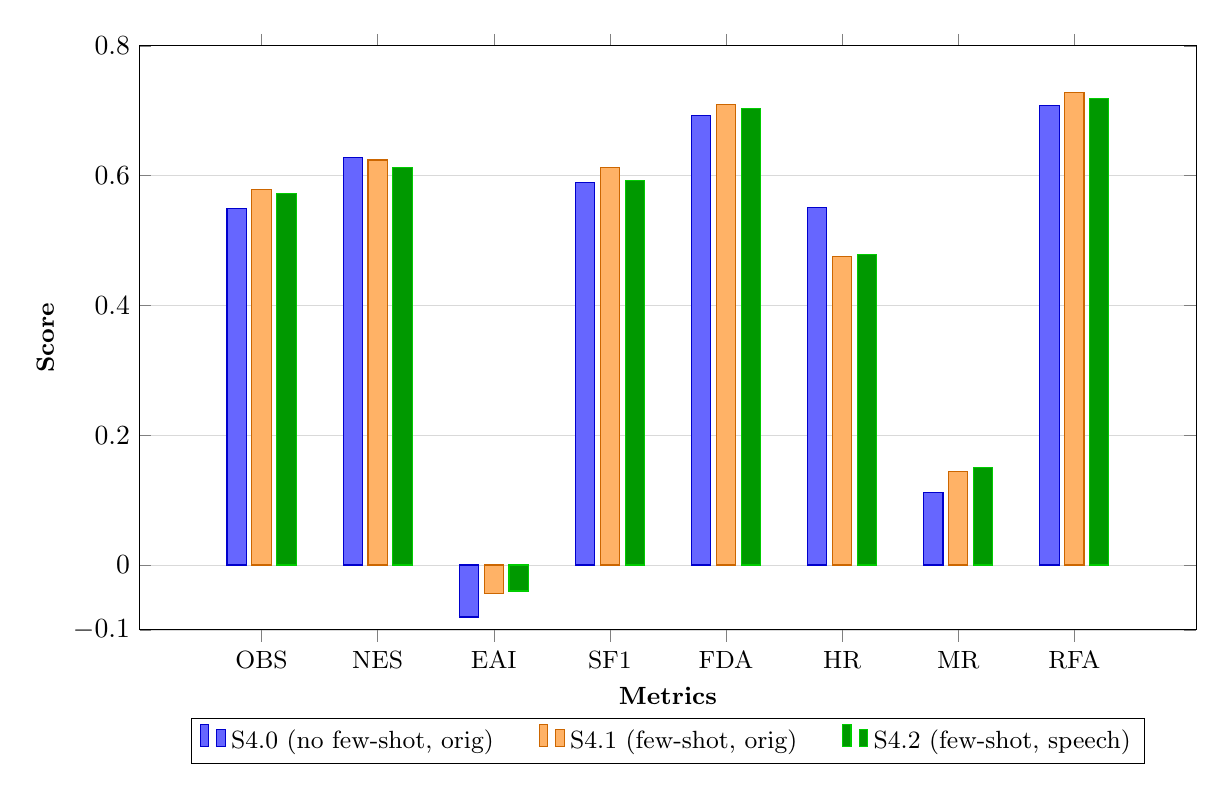
\begin{tikzpicture}
  \begin{axis}[
    width=15cm,
    height=9cm,
    ybar,
    bar width=7pt,
    ylabel={Score},
    ylabel style={font=\small\bfseries},
    xlabel={Metrics},
    xlabel style={font=\small\bfseries},
    symbolic x coords={OBS, NES, EAI, SF1, FDA, HR, MR, RFA},
    xtick=data,
    xticklabel style={font=\small},
    ymin=-0.1,
    ymax=0.8,
    ytick={-0.1, 0, 0.2, 0.4, 0.6, 0.8},
    ymajorgrids=true,
    grid style={line width=0.3pt, draw=gray!30},
    legend style={
      at={(0.5,-0.15)},
      anchor=north,
      legend columns=3,
      font=\small,
      /tikz/every even column/.append style={column sep=0.5cm}
    },
    enlarge x limits=0.15,
  ]
  
  % S4.0 (no few-shot, orig) - Blue
  \addplot[fill=blue!60, draw=blue!80!black] coordinates {
    (OBS, 0.549)
    (NES, 0.628)
    (EAI, -0.080)
    (SF1, 0.589)
    (FDA, 0.693)
    (HR, 0.551)
    (MR, 0.112)
    (RFA, 0.708)
  };
  \addlegendentry{S4.0 (no few-shot, orig)}
  
  % S4.1 (few-shot, orig) - Orange
  \addplot[fill=orange!60, draw=orange!80!black] coordinates {
    (OBS, 0.579)
    (NES, 0.624)
    (EAI, -0.044)
    (SF1, 0.613)
    (FDA, 0.709)
    (HR, 0.476)
    (MR, 0.144)
    (RFA, 0.728)
  };
  \addlegendentry{S4.1 (few-shot, orig)}
  
  % S4.2 (few-shot, speech) - Green
  \addplot[fill=green!60!black, draw=green!80!black] coordinates {
    (OBS, 0.572)
    (NES, 0.612)
    (EAI, -0.040)
    (SF1, 0.592)
    (FDA, 0.704)
    (HR, 0.479)
    (MR, 0.150)
    (RFA, 0.719)
  };
  \addlegendentry{S4.2 (few-shot, speech)}
  
  \end{axis}
\end{tikzpicture}
\caption{Headline metrics for S4 variants on MUC-4 ($N{=}100$). 
The figure compares the performance of the multi-LLM per-field strategy under three 
configurations: S4.0 (no few-shot), S4.1 (few-shot), and S4.2 (few-shot with 
speech-style input). Few-shot prompting (S4.1) improves most accuracy-related metrics 
(OBS, SF1, FDA, RFA) but still yields negative EAI values, reflecting inconsistencies 
in model agreement at the slot level. The speech-style variant (S4.2) remains close to 
S4.1, suggesting that field-wise consensus helps buffer against noise introduced by 
ASR-like phrasing. Overall, S4 demonstrates strong schema adherence but shows that 
per-field aggregation can amplify model disagreement in certain categories.}

\label{fig:s4-variants-bar}
\end{figure}


Per-field consensus boosts \texttt{incidentLocation}; \texttt{perpetratorIndividual} remains hardest; \texttt{weapon} is lower than in S1 and S3.

Figure ~\ref{fig:s4-perfield-plo} illustrates the asymmetric effects of per-field voting on different slots. \texttt{incidentLocation} benefits most, reaching an average score of $0.641$ in S4.1 and surpassing the corresponding values in the single-pass and full-document consensus strategies, which suggests that slot-specific prompts plus ensemble agreement help to stabilise location predictions. \texttt{incidentStage} also performs strongly ($0.720$), consistent with its comparatively structured label space. In contrast, \texttt{incidentType} and especially \texttt{incidentDate} underperform relative to other strategies (down to $0.370$ for dates), which indicates that aggressive filling at the field level can lead to more spurious or partially incorrect outputs when the signal is weak. \texttt{weapon} achieves $0.692$, clearly lower than in S1 and S3, suggesting that per-field voting may over-accept marginal mentions and noise in this slot. \texttt{perpetratorIndividual} remains one of the hardest fields despite the richer consensus mechanism, reflecting the persistent difficulty of sparse, ambiguous references to individual actors.

\begin{figure}[H]
\centering
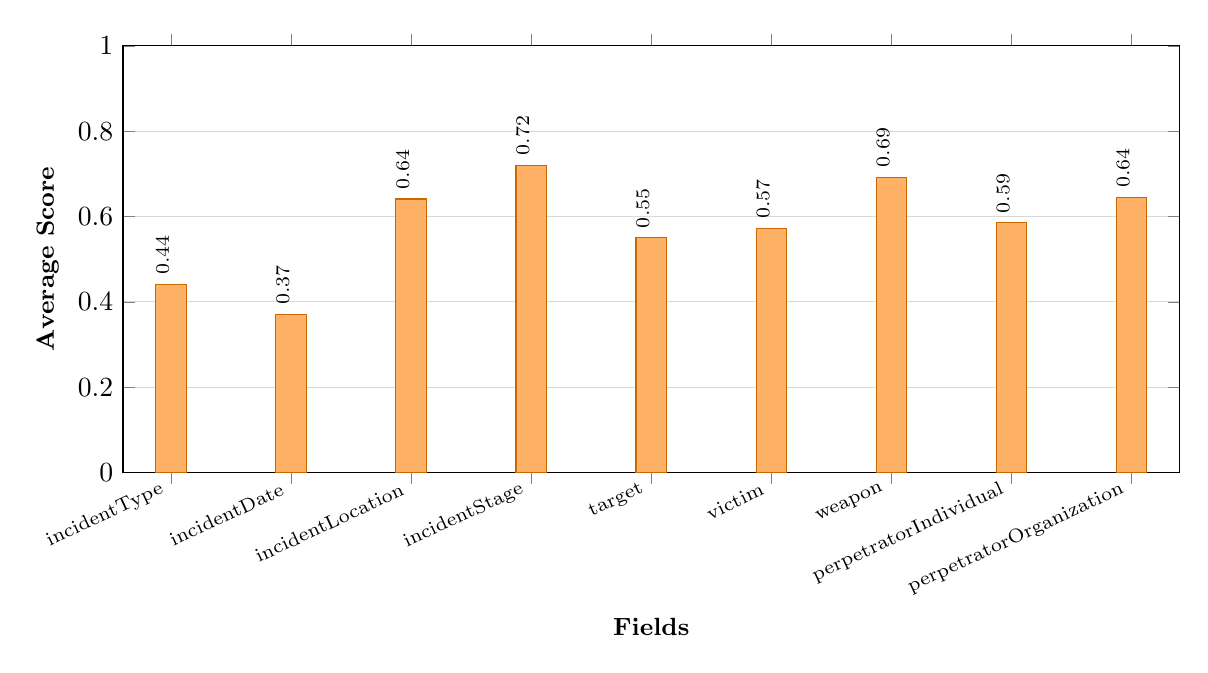
\begin{tikzpicture}
  \begin{axis}[
    width=15cm,
    height=7cm,
    ybar,
    bar width=11pt,
    ylabel={Average Score},
    ylabel style={font=\small\bfseries},
    xlabel={Fields},
    xlabel style={font=\small\bfseries},
    symbolic x coords={
      incidentType,
      incidentDate,
      incidentLocation,
      incidentStage,
      target,
      victim,
      weapon,
      perpetratorIndividual,
      perpetratorOrganization
    },
    xtick=data,
    xticklabel style={font=\scriptsize, rotate=25, anchor=east},
    ymin=0,
    ymax=1.0,
    ymajorgrids=true,
    grid style={line width=0.3pt, draw=gray!30},
    enlarge x limits=0.05,
    nodes near coords,
    nodes near coords style={
        font=\scriptsize,
        rotate=90,
        anchor=west,
        yshift=3pt
    }
  ]

  \addplot[fill=orange!60, draw=orange!80!black] coordinates {
    (incidentType, 0.440)
    (incidentDate, 0.370)
    (incidentLocation, 0.641)
    (incidentStage, 0.720)
    (target, 0.550)
    (victim, 0.572)
    (weapon, 0.692)
    (perpetratorIndividual, 0.585)
    (perpetratorOrganization, 0.644)
  };

  \end{axis}
\end{tikzpicture}

\caption{Per-field extraction performance for S4.1 on the MUC-4 subset ($N{=}100$). 
The multi-LLM per-field strategy shows strong results on structured categories such as 
\textit{incidentStage}, \textit{weapon}, and \textit{incidentLocation}, but performs noticeably 
worse on \textit{incidentType} and \textit{incidentDate}. These patterns indicate that while 
per-field consensus helps stabilize some slots, it also amplifies disagreement or uncertainty 
in fields that require broader contextual reasoning. Overall, S4.1 provides a mixed profile 
with clear strengths in schema-aligned attributes and weaknesses in categories involving 
interpretation or ambiguity.}
\label{fig:s4-perfield-plot}
\end{figure}


\subsection*{Latency}

\begin{figure}[H]
\centering
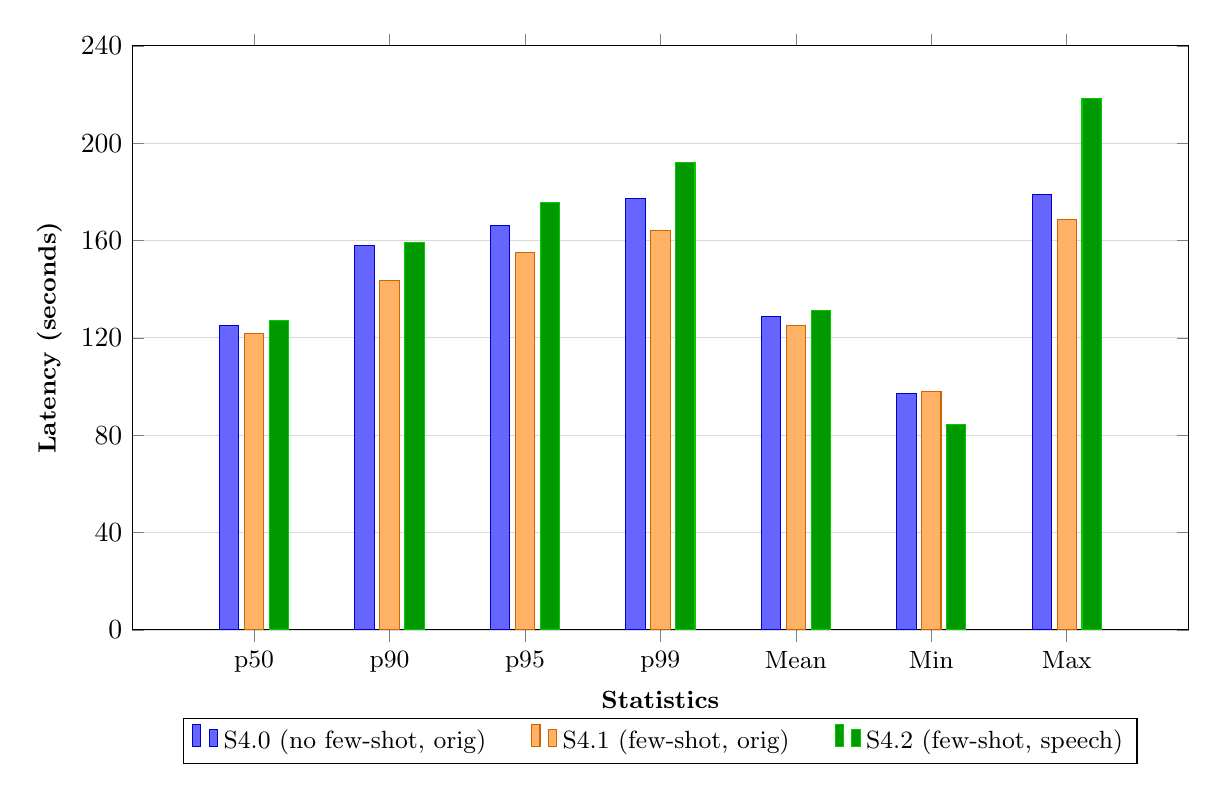
\begin{tikzpicture}
  \begin{axis}[
    width=15cm,
    height=9cm,
    ybar,
    bar width=7pt,
    ylabel={Latency (seconds)},
    ylabel style={font=\small\bfseries},
    xlabel={Statistics},
    xlabel style={font=\small\bfseries},
    symbolic x coords={p50, p90, p95, p99, Mean, Min, Max},
    xtick=data,
    xticklabel style={font=\small},
    ymin=0,
    ymax=240,
    ytick={0, 40, 80, 120, 160, 200, 240},
    ymajorgrids=true,
    grid style={line width=0.3pt, draw=gray!30},
    legend style={
      at={(0.5,-0.15)},
      anchor=north,
      legend columns=3,
      font=\small,
      /tikz/every even column/.append style={column sep=0.5cm}
    },
    enlarge x limits=0.15,
  ]
  
  % S4.0 (no few-shot, orig) - Blue
  \addplot[fill=blue!60, draw=blue!80!black] coordinates {
    (p50, 125.14)
    (p90, 157.96)
    (p95, 166.02)
    (p99, 177.27)
    (Mean, 128.64)
    (Min, 97.08)
    (Max, 179.00)
  };
  \addlegendentry{S4.0 (no few-shot, orig)}
  
  % S4.1 (few-shot, orig) - Orange
  \addplot[fill=orange!60, draw=orange!80!black] coordinates {
    (p50, 121.81)
    (p90, 143.39)
    (p95, 155.16)
    (p99, 164.08)
    (Mean, 124.98)
    (Min, 98.10)
    (Max, 168.81)
  };
  \addlegendentry{S4.1 (few-shot, orig)}
  
  % S4.2 (few-shot, speech) - Green
  \addplot[fill=green!60!black, draw=green!80!black] coordinates {
    (p50, 127.23)
    (p90, 159.02)
    (p95, 175.50)
    (p99, 192.16)
    (Mean, 131.15)
    (Min, 84.42)
    (Max, 218.22)
  };
  \addlegendentry{S4.2 (few-shot, speech)}
  
  \end{axis}
\end{tikzpicture}
\caption{Latency statistics for S4 variants (seconds). 
The per-field multi-LLM strategy incurs the highest computational cost among all evaluated 
approaches, with median latencies around 2 minutes and p99 values approaching or exceeding 
3 minutes. Few-shot prompting (S4.1) slightly reduces extreme latencies compared to the 
no–few-shot baseline (S4.0), likely due to more stable extraction behavior across models. 
The speech-style input (S4.2), however, introduces greater variance and higher worst-case 
latencies. Overall, S4 highlights the trade-off between robustness gained through 
per-field consensus and the substantial runtime overhead required for multiple coordinated 
LLM calls.}

\label{fig:s4-latency-bar}
\end{figure}

Figure~\ref{fig:s4-latency-bar} makes clear that S4 is the slowest strategy family. All three variants have median latencies in the 122–127\,s range per document and heavy upper tails, with p99 values between roughly $164$\,s and $192$\,s. This behaviour is expected because S4 runs multiple models for each individual slot rather than once per document. Few-shot prompting slightly reduces median and mean latency when moving from S4.0 to S4.1, but the differences are small compared to the overall cost of per-field ensemble processing. S4.2 is marginally slower than S4.1 on average and exhibits the heaviest tail (Max above $218$\,s), reflecting additional variability in convergence on speech-style inputs. In comparison to S3.1, which also uses multi-LLM consensus but at the document level, S4 sacrifices throughput for more aggressive slot-level filling; this makes it less attractive for high-volume or time-sensitive deployments unless very high recall on nonempty fields is the primary objective.

\subsection*{Cost Analysis (S4: Multi-LLM Per-Field Consensus)}

\textbf{Assumptions.} For each of the $F{=}9$ fields, two parallel extractions are run—\textit{GPT-5} and \textit{Gemini~2.5~Pro}—with per-field averages $i_f{=}1{,}500$ input tokens and $o_f{=}50$ output tokens. A single arbiter/verification step per record runs on \textit{GPT-5-mini} with $V_{\text{in}}{=}1{,}000$ and $V_{\text{out}}{=}100$. If audio is used, Whisper transcription for $D$ minutes is added once per record.

\textbf{Prices.} GPT-5: input \$1.25/M, output \$10.00/M. Gemini~2.5~Pro: input \$1.25/M, output \$10.00/M. GPT-5-mini: input \$0.25/M, output \$2.00/M. Whisper: \$0.006/min.

\textbf{Formula.}
\[
\text{Cost}_{\text{S4}} =
\sum_{f=1}^{F}\!\Big[
\underbrace{\tfrac{i_f}{10^6}p_{\text{in}}^{(5)} + \tfrac{o_f}{10^6}p_{\text{out}}^{(5)}}_{\text{GPT-5 per field}}
+
\underbrace{\tfrac{i_f}{10^6}p_{\text{in}}^{(\text{Gemini})} + \tfrac{o_f}{10^6}p_{\text{out}}^{(\text{Gemini})}}_{\text{Gemini per field}}
\Big]
+\underbrace{\tfrac{V_{\text{in}}}{10^6}p_{\text{in}}^{(\text{mini})}+\tfrac{V_{\text{out}}}{10^6}p_{\text{out}}^{(\text{mini})}}_{\text{single arbiter}}
+0.006\cdot D
\]

\textbf{Per-record (no audio).}
\[
\begin{aligned}
\text{Per field (GPT-5): } & \tfrac{1500}{10^6}\!\cdot\!1.25 + \tfrac{50}{10^6}\!\cdot\!10.00 = \$0.002375 \\
\text{Per field (Gemini): } & \tfrac{1500}{10^6}\!\cdot\!1.25 + \tfrac{50}{10^6}\!\cdot\!10.00 = \$0.002375 \\
\text{Both models per field: } & \$0.00475 \\
\text{Across }F{=}9\text{ fields: } & 9 \times 0.00475 = \$0.04275 \\
\text{Arbiter (mini, once): } & \tfrac{1000}{10^6}\!\cdot\!0.25 + \tfrac{100}{10^6}\!\cdot\!2.00 = \$0.00045 \\
\textbf{Total: } & \mathbf{\$0.04320}\ (\approx 4.32\text{¢/doc})
\end{aligned}
\]

\textbf{With audio (Whisper).} Adding Whisper introduces a linear term $0.006\cdot D$. For $D{=}1$\,min, the total cost becomes $\$0.04320 + 0.006 = \mathbf{\$0.04920}$ (approximately $4.92$\,¢ per document). At these settings, S4 costs about $6\times$ as much as S1 (\$0.04320 vs.\ \$0.00720 per document, no audio) and roughly $2\times$ as much as S2 (\$0.04320 vs.\ \$0.02183), with the main driver being the per-field dual-model passes; the single-record arbiter remains a relatively minor component of the overall cost.

\subsection*{Consistency (Formatting \& Style)}

Figure~\ref{fig:s4-consistency} shows that S4 maintains reasonably high structural and stylistic consistency despite its aggressive fill behaviour. All variants achieve $\mathrm{FPR}_{\text{overall}}$ above $0.87$, and few-shot prompting again helps: S4.1 and S4.2 reach $0.94$, closing most of the gap to the best-performing strategies in this regard. Style-aware consistency $\mathrm{SC}_{\text{macro}}$ increases from $0.6599$ in S4.0 to $0.6881$ in S4.1, with a small drop to $0.6815$ for S4.2 on speech-style input. This suggests that the combination of per-slot prompting and consensus does not destabilise output formatting, even though the model ensemble is more willing to produce content in marginal cases.

Taken together, the S4 results characterise multi-LLM per-field consensus as an aggressive, recall-oriented strategy. It achieves high NES and strong performance on genuinely nonempty slots, particularly for context-sensitive fields such as \texttt{incidentLocation}, but this comes at the cost of elevated hallucination rates, negative EAI, and substantially higher latency and monetary cost. Compared to full-document consensus (S3.1), S4.1 offers higher NES (0.624 vs.\ 0.521) but lower OBS (0.579 vs.\ 0.641) because it overfills when gold is empty. In scenarios where maximising content recall on nonempty slots is critical and throughput is less of a concern, S4.1 is a compelling option—especially if combined with downstream post-filters. For more balanced deployments that must trade off accuracy, calibration, latency, and cost, S3.1 provides a more favourable operating point than S4’s per-field ensemble.```

\begin{figure}[H]
\centering
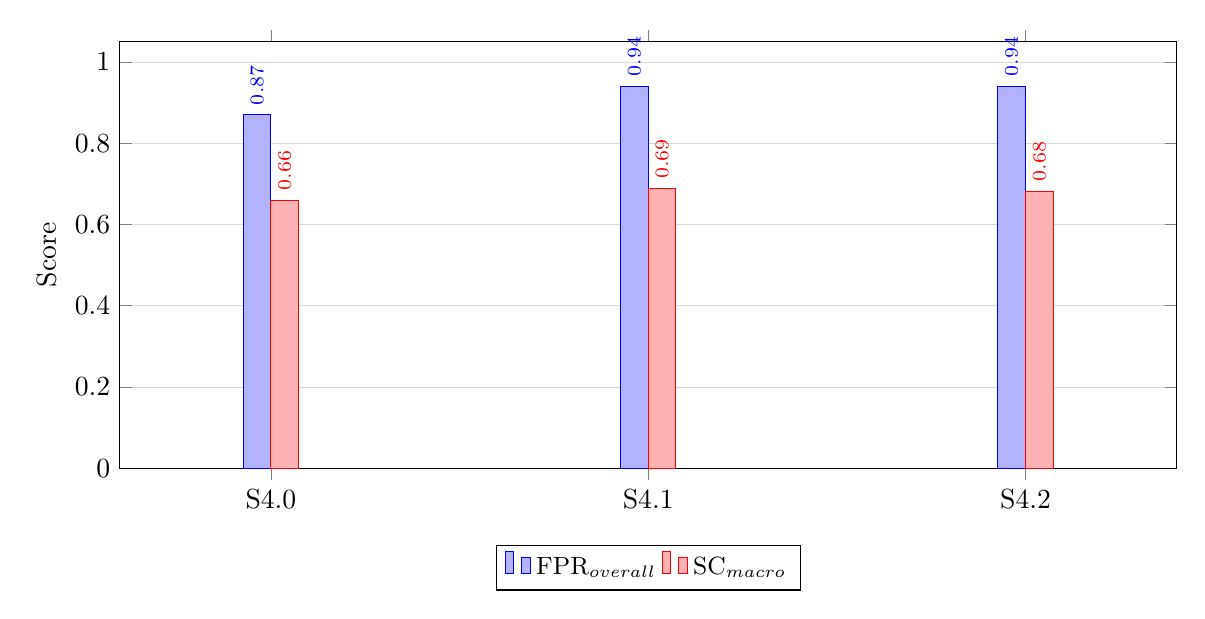
\begin{tikzpicture}
  \begin{axis}[
    width=15cm,
    height=7cm,
    ybar=0pt,
    bar width=10pt,
    ymin=0, ymax=1.05,
    ylabel={Score},
    symbolic x coords={S4.0,S4.1,S4.2},
    xtick=data,
    ymajorgrids=true,
    grid style={line width=0.3pt, draw=gray!30},
    legend style={at={(0.5,-0.18)}, anchor=north, legend columns=2, font=\small},
    enlarge x limits=0.20,
    nodes near coords,
    nodes near coords style={
        font=\scriptsize,
        rotate=90,     % vertical text
        anchor=west,
    }
  ]
    % FPR_overall
    \addplot coordinates {(S4.0,0.870) (S4.1,0.940) (S4.2,0.940)};
    \addlegendentry{$\mathrm{FPR}_{\text{overall}}$}

    % SC_macro
    \addplot coordinates {(S4.0,0.6599) (S4.1,0.6881) (S4.2,0.6815)};
    \addlegendentry{$\mathrm{SC}_{\text{macro}}$}
  \end{axis}
\end{tikzpicture}
\caption{Consistency (S4 variants): schema formatting vs.\ input-aware style.}
\label{fig:s4-consistency}
\end{figure}

